%%
\chapter{Design time details}
%%



Before the monitoring components can be deployed we 



\section{Overview of the query compilation workflow}

The compilation of the queries of the CPS is depicted in fig. \ref{figure:query-compile-workflow}. First the local search planner of the \viatra{} system creates a plan. We complete the generated plan with types and other supplementary information, and make a distributed version of the plans. After that, we use additional optimization specialized for our execution mechanism to improve the execution. After the fully optimized plan is ready, we can construct the generator model describing the source code structure and generate the \cpp{} files.

\begin{figure}[h]
	\begin{center}
		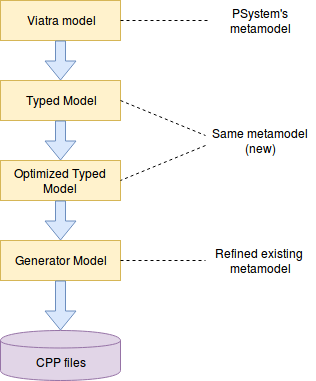
\includegraphics[width=0.5\textwidth]{figures/workflow.png}
		\caption{Query comompilation workflow}
		\label{figure:query-compile-workflow}
	\end{center}
\end{figure}


\section{Viatra plan}


\section{Completed plan}


\section{Additional optimization}


\section{C++ code generation}


